\section{Methods}

Our methodology is based on the implementation of a complete data cycle
to enhance model predictions in a coastal ocean domain through robotic
adaptive sampling and data assimilation. The approach consists of three
fundamental steps, executed iteratively on a daily basis:

\begin{description}

\item[Model Forecast and Uncertainty Projection]: A numerical ocean
  model provides a daily one-step forecast $\hat{\theta}(k+1, x, y)$
  of a target oceanic variable $\theta$, along with an associated
  uncertainty field $\sigma_{\hat{\theta}}(k+1, x, y)$, where $k$
  represents the current day and $(x, y)$ denote the geographical
  coordinates.  These outputs are organized into discrete spatial
  maps, $M_{\hat{\theta}}(x, y)$ and
  $M_{\sigma_{\hat{\theta}}}(x, y)$, representing, respectively, the
  predicted state and its uncertainty over a predefined grid covering
  the study area.
    
\item \textbf{Target Sample Planning}: Using the uncertainty map
  $M_{\sigma_{\hat{\theta}}}(x, y)$ as input, a targeted sampling
  algorithm determines the set of trajectories for a fleet of $N$ AUVs
  for the next operational cycle. The goal is to maximize the
  accumulated uncertainty sampled along the vehicle paths, while
  satisfying vehicle-specific constraints. The planned trajectories
  are transmitted to the vehicles for execution.

\item \textbf{Data Collection and Assimilation}: Throughout the
  operational period, each AUV collects measurements of the target
  variable $\theta$ along its assigned path. After the mission is
  completed, the collected measurements are assimilated into the
  numerical model using an appropriate data assimilation scheme. This
  updated model state serves as the new initial condition for the next
  forecasting cycle, closing the loop.

\end{description}

While previous efforts have concentrated on a form on embedded
automated decision-making on AUVs
\cite{mcgann08a,mcgann08b,ryan10,py10,Das-2010-637,das10,olaya12,rajan12}
to demonstrate adaptive sampling, here we AUV trajectories are defined
by human-in-the-loop decisions apriori, with adaptation focused on
deployment based on $M_{\sigma_{\hat{\theta}}}(x, y)$. No automated
decisions were made on the AUVs. Loop closure in this work, refers to
the \emph{sample-assimilate-predict-direct} process as indicated in
Fig. \ref{fig:loop-closure}.

\subsection{Model Forecast and Uncertainty Projection}

Sampling strategies rely on timely information about the spatial
variability of ocean properties. However, conventional numerical ocean
models are computationally intensive, and their runtime makes them
impractical for use in near-real-time mission planning \krcom{Need a
  citation here}. While similar assimilation cycles could in principle
be implemented directly within deterministic numerical models, this
would require either substantially higher computational resources or
larger temporal horizons. As a more practical alternative, we employ
geostatistical simulation as a computationally efficient surrogate,
producing short-term predictions of ocean temperature together with
estimates of uncertainty \cite{deutsch1992}. This approach captures
the essential variability of local ocean dynamics at a fraction of the
cost of full numerical models, while remaining flexible enough to
assimilate new in situ observations quickly \cite{Duarte2025} and
coherent with the scope of the work approach.

The methodology relies on ensembles of geostatistical realizations, each
representing a state of the ocean temperature field conditioned by a
priori deterministic ocean models \cite{CMEMS2017} and direct
observations. By computing the pointwise standard deviation across the
ensemble, we obtain spatial uncertainty maps that highlight regions
where predictions are less constrained and potentially more informative
for sampling. These maps serve as the basis for identifying areas where
new measurements are expected to maximize the reduction of forecast
error \cite{Duarte2025}.

Geostatistical realizations are produced using direct sequential
simulation \cite{soares2001direct}, a stochastic method that draws
values from conditional probability distributions defined by kriging
estimates and variances. The continuity of the temperature field in
space and time is characterized by variogram models fitted to long-term
calibrated ocean model data \cite{CMEMS2017}. At each depth, simulations
are carried out independently, using a moving temporal window of
fourteen previous days to predict the subsequent day. This
sliding-window strategy strikes a balance between forecast skill and
computational feasibility, and can be adapted according to the
complexity of the oceanographic conditions.

The ensemble of realisations provides both a forecast of ocean
temperature and a quantitative assessment of the prediction
uncertainty.  By updating the forecasts with new AUV measurements
through sequential assimilation, the method progressively refines the
temperature field while maintaining consistency with prior model
dynamics. The resulting forecasts and uncertainty maps form the input
for the target sampling algorithm, guiding the allocation of AUV
trajectories towards regions of greatest expected information
gain. More details about the model, its development, and application
during the \proj experiment can be found in \cite{Duarte2025}.

\subsection{Target Sampling Algorithm}

The adaptive sampling problem here is posed as the design of vehicle
trajectories that maximize information gain
\cite{eidsvik2015,fossum18} extracted from a model-derived uncertainty
map, while satisfying operational AUV constraints. Each day, the
models provide both a forecast field and its associated uncertainty
distribution, which together define the reward landscape for the
planner. The task is then to generate, for each vehicle, a path
composed of waypoints that accumulates the highest possible
uncertainty values.

To address this, the problem is cast as a graph theoretic problem. The
spatial uncertainty map is first pre-processed to remove obstacles and
smoothened to highlight large-scale features. Candidate waypoints are
then identified from the map and used to build a weighted graph, where
nodes carry a reward proportional to their uncertainty value and edges
represent travel costs. The trajectory planning task is posed as a
Prize Collecting Vehicle Routing Problem
(PCVRP)\cite{vidal2013,toth2014vehicle} where routes must balance the
rewards obtained from visiting nodes with associated costs of
traveling between them. By solving this, the algorithm returns a set
of near-optimal trajectories that prioritize regions of greatest
uncertainty, while ensuring vehicle endurance and safety
constraints. This provides a principled way of steering autonomous
platforms toward the most informative sampling locations, forming a
key component in the daily cycle of forecast, adaptive sampling, and
data assimilation. Additional insights into the algorithm and its
deployment during \proj are reported elsewhere in
\cite{bernacchi2025}.

\subsection{Data Collection}

\subsubsection{System of systems for ocean observation}

TO DECIDE:
\begin{itemize}
    \item INCLUDE IH explaining that here we are focused on auv data
    \item check for the definition of C2 for the first time
    \item PRESENT EXAMPLES OF RIPPLES LAYERS HERE OR REFER TO OTHER SECTIONS WERE THOSE MAY BE DISPLAYED
    \item INCLUDE MODEL AND MAKE OF SENSORS
\end{itemize}

The System of Systems for ocean observation deployed in this field study
comprised systems contributed by the LSTS, the Hydrographic Institute
(IH), Portuguese Navy, and the University of Columbia.

IH deployed the NRP \emph{D. Carlos} oceanographic vessel contributing
wet laboratories, a rosette equipped with CTDs, Niskin bottles and an
Underwater Vision
Profiler %(http://www.hydroptic.com/index.php/public/Page/product_item/UVP6-LP)%,
and an Alseamar Glider equipped with a
CTD %(https://www.alseamar-alcen.com/ocean-science-sector/seaexplorer-gliders/seaexplorer-1000/)%.

LSTS deployed 5 Xplore long endurance AUVs along with 6 Manta
communication gateways (Figure \ref{fig:lauvs}) and control stations for
the field experiments in Nazaré. The Xplore class AUV \cite{lauvurl} is
an AUV designed for water column operations equipped with CTD,
fluorometer, turbidity, O2, cameras, and nutrient sensors, WiFi and
satellite communications (Iridium), acoustic modems, and battery packs
enabling 60h+ endurance. The CTDs mounted on the AUVs were calibrated
and cross-calibrated at IH calibration facilities. The Manta
communication gateways \cite{} are equipped with acoustic modems,
satellite and Wi-Fi modules for long range communications with
underwater, surface, and aerial vehicles. The AUV operations were
supported by two boats rented in Nazaré. In addition, to the existing
command and control center located in Porto, LSTS installed another in
Nazaré. Two Manta units were installed in the support boats to support
local deployments and communications with the command and control
centers. Four units were used to support the command and control center
installed in Nazaré.

\begin{figure}
    \centering
    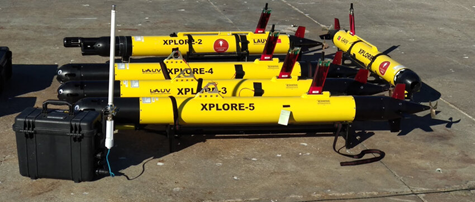
\includegraphics[width=.7\linewidth]{fig/lauvs.png}
    \caption{The AUVs deployed in the experiment.}
    \label{fig:lauvs}
\end{figure}


The Columbia University deployed a vertical profiler equipped with a CTD
and portable CTD deployed from the support boats.

The Xplore AUVs, control stations, and Manta gateways were powered by
the LSTS software toolchain \cite{pinto2013lsts} deploying command and
control, data pipelines, and algorithm integration to support closing
the modeling-sample-assimilation-tasking cycles. The 4 components of the
toolchain are briefly described below:

DUNE, the onboard control software, running on vehicles and other
devices. DUNE interfaces with sensors and actuators, by sending commands
and monitoring them. DUNE is also in charge of executing missions and
commands sent by the command and control (C2) stations. DUNE and its
upper water column backseat implementation provided additional
functionally for Iridium satellite communications, telemetry, and
interaction with Neptus.

IMC, the messaging protocol. It includes a definition of messages and
its serialization. It is used to send and receive commands and data
between vehicles and the C2 stations. A few IMC messages were created to
support this field experiment. NEPTUS, the C2 software framework. Neptus
presents a graphical user interface (GUI) enabling the operator to
connect to one or several heterogeneous vehicles (underwater, surface,
aerial, or sensors). With Neptus, one operator can control multiple
vehicles simultaneously, sending commands, missions, and receiving and
monitoring telemetry and data using Wi-Fi acoustics, or satellite
communications. For this deployment Neptus incorporated new developments
to streamline the integration of telemetry coming through the Iridium
satellite communications with existing GUIs and to import optimal routes
generated by the adaptive sampling algorithm into mission plans to send
to the vehicles.

RIPPLES, the Web based C2 that supports situational awareness of
unmanned systems operations. It supports real-time monitoring of an
operation and planning of such operations by providing access to several
data products layers. These layers include environmental data and other
support models for the environment and additions marine traffic in the
vicinity of the operating autonomous vehicles (such AIS and aircraft
data, or density maps). New layers were added to RIPPLES to support new
aspects planning and execution control for this deployment.

Figure XXX shows outputs of the HOPS (Harvard Ocean Prediction System)
with temperature and salinity model outputs and respective errors.
Another layer displayed geostatistical model outputs XXX. These outputs
were used to monitor progress by enabling the visualization of updated
during the execution of the operation.

IH has several buoys in the area. A new layer to directly access and
visualize their data in real-time was added to RIPPLES (Figure
\ref{fig:buoys}. This provided wave information for the area (real-time
and historical).


\begin{figure}
    \centering
    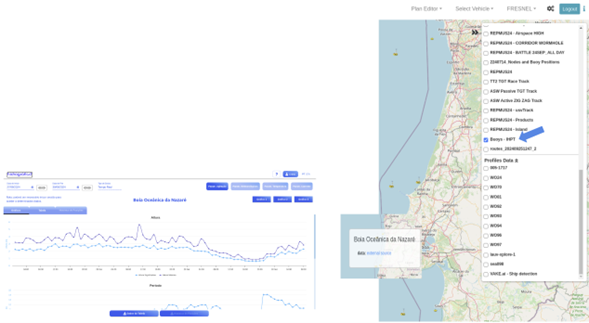
\includegraphics[width=.7\linewidth]{fig/buoys.png}
    \caption{AUVs deployed in the experiment.}
    \label{fibuoys}
\end{figure}

 
Optimal routes were generated for the AUVs to execute. A new Ripples
layer enabled the user to visualize all the routes taken by the AUVs, as
well as the routes generated for future deployments. This contributed to
a timely launch and deployment of the vehicles.
 
New layers for the visualization of remote sensing data, as well as of
data collected by sensors installed onboard NRP D. Carlos were also
deployed.


% The adaptive sampling problem is formulated as an optimization task
% aiming to maximize the expected information gain from the
% observations. Specifically, given the predicted uncertainty map and
% operational constraints (e.g., time, energy budget), the algorithm
% plans vehicle routes that prioritize areas of higher model
% uncertainty. The uncertainty along each candidate path is evaluated,
% and path planning strategies — such as greedy heuristics or
% combinatorial optimization techniques — are employed to allocate
% waypoints efficiently among the available AUVs.

\subsubsection{Field deployment: planning and preparation}

IH contributed the NRP D. Carlos for 5 days during one of the planned
offshore buoy maintenance missions taking place annually in April or in
October. The October period was selected for the \proj deployment. The
meteorological and ocean conditions are typically not significantly
different in these periods and may be affected by distant storms taking
place in the Atlantic.

The planned time window for the \proj deployment with NRP D. Carlos was
the second week of October. However, this time window had to be shifted
by one week, to start October 20th, because of challenging
meteorological and ocean conditions. The AUV deployments were planned to
start the first week of October but were delayed starting October 14th
and end October 31st. The decisions to delay both the ship and AUV
deployments proved to be adequate and made it possible to have 5 days of
ship time and 7 days of AUV operations. This also enabled concurrent
operations of the ship, glider, and AUVs. The AUVs collected data one
week in advance of the ship’s arrival and kept running the developed
algorithms during the third week of the deployment. The planned areas of
operation for NRP D. Carlos (large rectangle) and for the AUVs (smaller
rectangle) are depicted next.

\begin{figure}
    \centering
    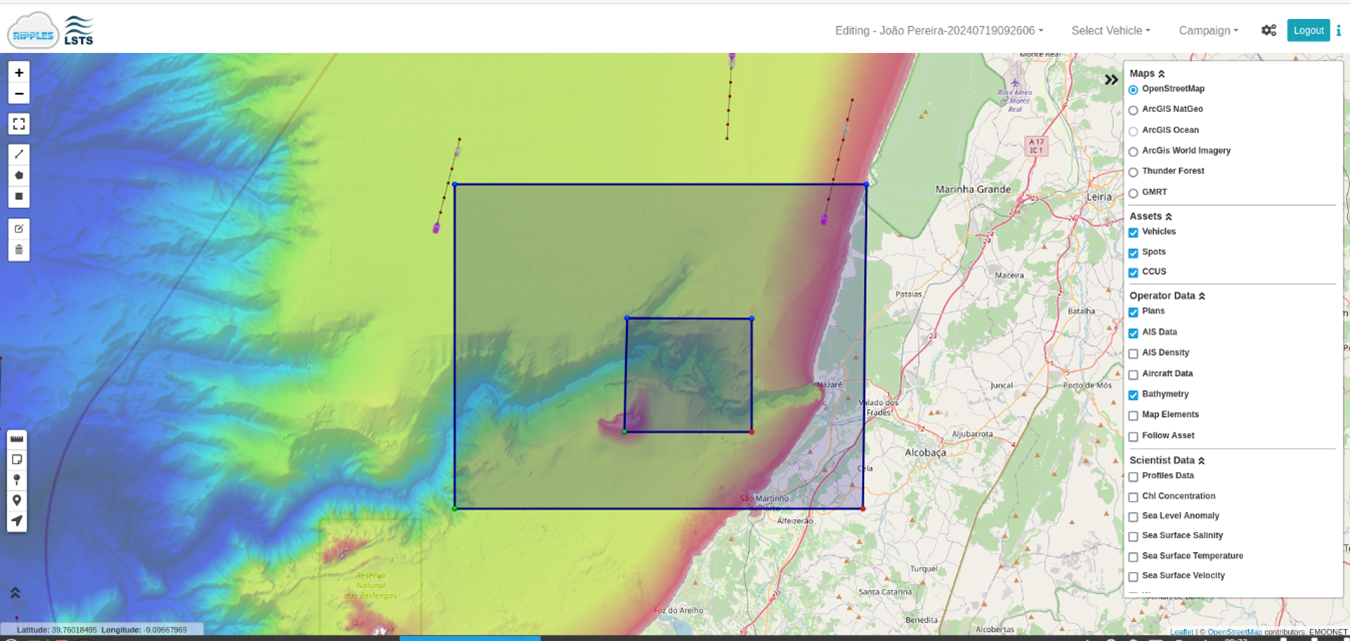
\includegraphics[width=.7\linewidth]{fig/Opareaas.png}
    \caption{Areas of operations for NRP D. Carlos and for the AUVs.}
    \label{fig:opareas}
\end{figure}

These areas have intense ship traffic, particularly from fishing
vessels, that presents added collision risks to AUVs at surface or when
surfacing, as well as potential encounters with bottom trawling fishing
nets. In addition, because Nazaré is a fishing harbor there is the added
challenge of AUV encounters with fishing nets.

To address these challenges we started by meeting fisherman associations
with the support of the city hall to engage the community, understand
their fishing procedures and the probable locations of fishing nets.
Second, we studied AIS patterns and densities, first for one year, then
for one month, and finally for each week in October. This enabled us to
partition the operations area into 3 areas with increasing risk levels
\ref{fig:riskareas}. We focused our operations on the first two areas,
starting operations at the one where risk was lower. Finally, by
studying daily patterns we were able to establish temporary areas for
operations with acceptable risks. We have distilled this knowledge into
operational procedures and automated decision aids and alerts.

\begin{figure}
    \centering
    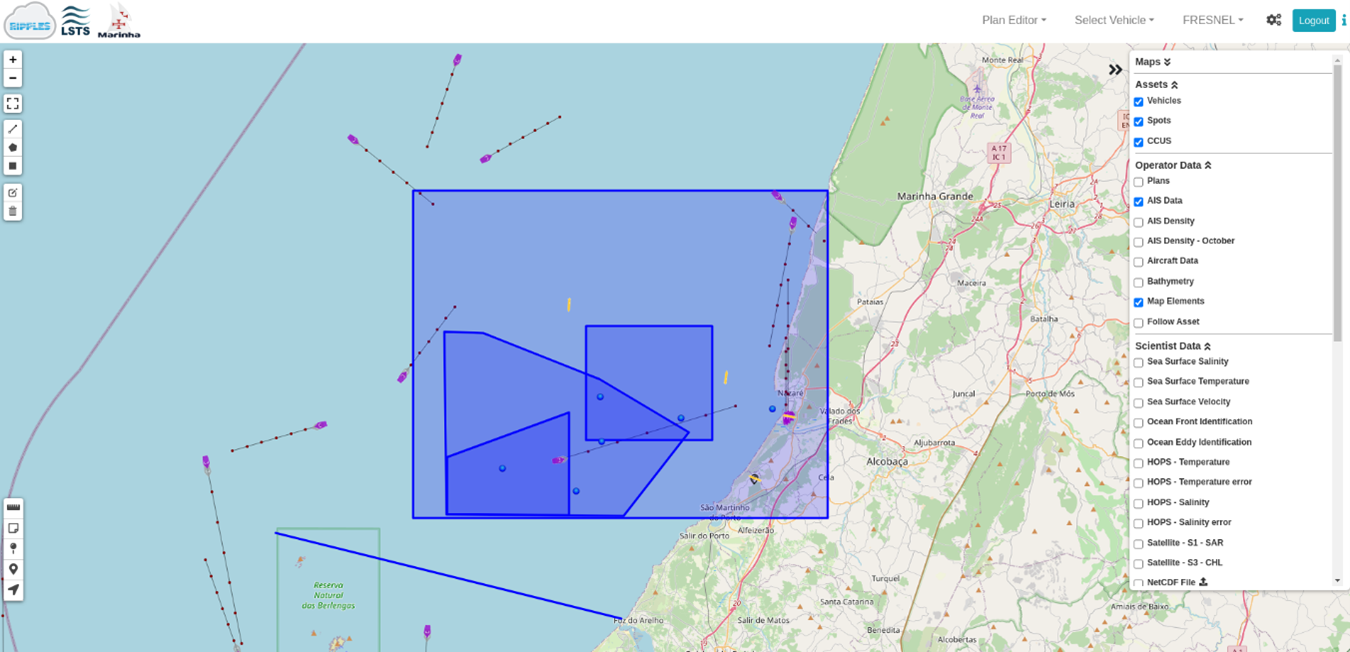
\includegraphics[width=.7\linewidth]{fig/riskareas.png}
    \caption{The operational area was partitioned into 3 areas with
      different levels of risk} XXX PLACE RISK MAP SIDE BY SIDE
    \label{fig:riskareas}
\end{figure}

Field operations were organized into two concurrent activities:

\begin{itemize}
\item NRP \emph{D. Carlos} campaign taking place October 20th – 24th.
  Team members from the University of Aveiro were onboard NRP D. Carlos
  to support operations with the UVP and wet laboratory operations. In
  addition to the rosette casts a glider was also deployed from the
  ship. The deployment of the glider along the western boundary of the
  operations area provided some of the initial conditions for the HOPS
  model. The rosette casts provided a course description of essential
  ocean variables in the larger area of operation. XXX Detailed
  descriptions of these activities are presented in Annexes E - H.

\item AUV deployments taking place October 14th - 31st. These
  deployments were supported by two boats rented in Nazaré. In addition
  to the AUV deployments by LSTS-UPorto, water samples were collected by
  researchers from Columbia University. These data collection activities
  provided a dense grip of data collection points. XXX Detailed
  descriptions of these activities are presented in Annexes D, F, G.

\end{itemize}

These two activities were conducted in coordination, namely in what
concerns water space management and sharing of model predictions, done
with the help of the LSTS toolchain and the underlying communication
infrastructure. Both activities run 24/x. In the case of the AUV
deployments the LSTS-UPorto team operated in 4 6-hour long shifts with
minimal operator’s footprint (one active and one backup operator).
Operations were run from a house rented in Nazaré and from LSTS in
Porto.


\subsubsection{Field deployment: summary of AUV and ship operations}

Questions:
\begin{itemize}
    \item explain yoyos
    \item include a more detailed description of daily ops with tables?
\end{itemize}


AUV daily operations started with the analysis of remote sensing data,
data collected during the previous 24h, forecasts of meteorological and
ocean condition, performance of the planning and execution control
algorithms, performance of the modeling-sample-assimilation-tasking
cycle (this was done during the last week of operations), and mission
updates provided by the operators in charge of the night shifts.

AUV operations’ planning then proceeded in 2 different time horizons:

\begin{itemize}

\item Plan for the day, including launch and recovery of
  vehicles, as well as boat operations. 

\item Plan for next 2-3 days (3 AUVs could operate for 50h+). This was
  particularly challenging
  because it included calculating time of recovery and making sure that
  the meteorological and ocean conditions were feasible for these
  operations. AUV execution control was focused on addressing alerts
  (e.g., ships crossing the area of operations), coordinating launch and
  recovery of AUVs with the help of the two boats, and re-tasking the
  vehicles in case a significant change in the planning assumptions
  occurred. 

\end{itemize}

\proj operations started spanned October 14th - 31st period. We took a
risk-minimizing incremental approach to operations planning and
execution control. The first week was about getting acquainted with the
new area of operations and evaluating, testing, and improving
operational procedures. The second week was about deploying the whole
approach and learning from it. The third week focused on running AUV
operations to further evaluate and test the approach, namely in what
concerned simultaneous deployments and persistent observation.

The first week was about AUV and small boat operations (including
collecting water samples). The focus was on testing the validity of the
risk management approach (including the partition of the operations
area) and on evaluating and testing the operation of the AUVs in this
new area. AUV missions were already spanning at least 2-day durations.

The second week involved the 5-day long NRP \emph{D. Carlos} campaign
together with AUV operations with boat support for launch and recovery
and water sampling. Coordination of these concurrent operations involved
water space management, to prevent collisions, and ingestion of data
provided by the ship and AUVs for analysis and assimilation. The
experience acquired during this week was invaluable and provided the
templates for AUV operations taking place the following week. Over these
two weeks the AUVs were impacted several times by strong vertical
currents in areas of significant stratification. Our preliminary
analysis pointed to internal waves as the most probable cause of these
currents. The area is known for internal wave activity and remote
sensing data provided evidence of the presence of internal waves during
the same days.

The final week focused on AUV operations only. Multi-day AUV deployments
provided additional data about the modeling-sample-assimilation-tasking
cycle (executed several times). In addition, AUVs were deployed
concurrently not only in the area surveyed the previous week (to
minimize risk) but also in areas with higher risk of collisions in which
short time windows limited the duration of these deployments. This
required tighter planning and execution control procedures for the two
operators in charge of the concurrent operations. This is illustrated
with mission plans depicted in Figure \ref{fig:missionplans}. One AUV
was tasked to perform yo-yos along straight line (line in black) in an
area in which trawlers run North-South transects, while two others
performed the adaptive sampling algorithm further South in a safer area.
 
\begin{figure}
    \centering
    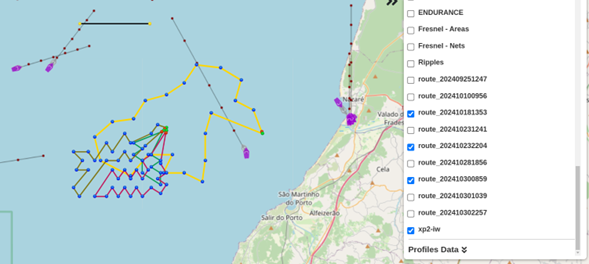
\includegraphics[width=.7\linewidth]{fig/missionplans.png}
    \caption{Example of mission plans (tours) to be executed by 3 AUVs.}
    \label{fig:missionplans}
\end{figure}


The AUV operators were provided with close to real-time information
about the data collected by the AUVs, as depicted in Figure
\ref{fig:temperatureprofiles} showing surfacing points for one mission
color-coded by temperature. The operator could click in any of these
points to get a temperature profile for the previous dive.

 \begin{figure}
    \centering
    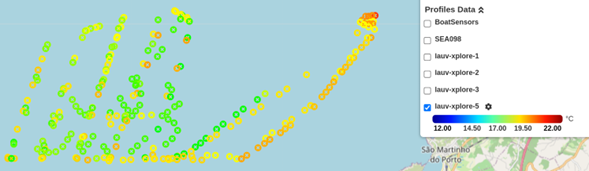
\includegraphics[width=.7\linewidth]{fig/temperatureprofiles.png}
    \caption{AUV path color-coded by levels of temperature at surfacing points.}
    \label{fig:temperatureprofiles}
\end{figure}



Despite the challenging meteorological and ocean conditions, that
strongly constrained the overall deployment, the \proj team was able to
demonstrate the overall approach during these 3 weeks (out of which only
7 days of operation were possible). The team operating the AUVs spent
these 3 weeks on site and on call to rapidly deploy or recover the AUVs
as dictated by meteorological and ocean conditions or forecasts.



\subsection{Field Experiment Analysis and Evaluation}

Although the FRESNEL field campaign extended over a longer period, for the purpose of this paper, only a three-day sequence of consecutive experiments (29–31 October) is considered, as it provides a representative demonstration of the proposed framework and its operational workflow.

The evaluation of the framework was carried out during the FRESNEL field campaign through a series of consecutive daily experiments designed to test the integration of model forecasts, target sampling planning, and data assimilation. All of these components were previously described. The analysis aimed to quantify the impact of assimilating AUV-acquired temperature data on the predictive performance of the statistical model and to assess the operational feasibility of the data cycle approach in a real-world coastal setting.

Each experimental day followed a structured cycle involving: (i) the generation of a statistical model forecast and its associated uncertainty field based on CMEMS data available up to the previous day; (ii) the execution of the target sampling algorithm to plan the next-day missions; and (iii) in situ data collection by the AUV fleet following the planned routes. The data collected within the previous day (0–24 h) were subsequently assimilated into the statistical model to produce updated forecasts, enabling comparisons between forecasts with and without data assimilation.

The campaign involved three Light Autonomous Underwater Vehicles (LAUVs) — Xplore2 (XP2), Xplore3 (XP3), and Xplore5 (XP5), which alternated daily in performing target sampling missions over the Nazaré Canyon region. On 29 October, the statistical model produced the initial forecast solution (A), which was used to plan the mission executed by XP2. The resulting in situ temperature data were later assimilated offline to produce an updated statistical model solution (B1) for 30 October. Although operational real-time assimilation was initially planned, logistical constraints prevented its implementation. Consequently, all assimilation cases were performed offline after mission completion. The target sampling algorithm, therefore, relied on statistical forecasts without assimilation (B), using pre-existing data as input for daily mission planning. This limitation is not expected to have significantly affected the experimental outcomes, as the operational area was spatially compact and the predicted variability field remained consistent between consecutive days. In future implementations, on-board or near-real-time assimilation should be considered to fully exploit the adaptive potential of the framework.

Data collected by XP3 and XP5 on 30 October were assimilated offline to generate new model solutions for 31 October (C1, C2, C3, C4), along with a non-assimilated reference case (C). The configurations were as follows:

\begin{itemize}
    \item C1 – assimilation including only XP2 data from 29 October;
    \item C2 – assimilation including XP2 (29 October) and XP5 (30 October) data;
    \item C3 – assimilation including only XP5 data from 30 October;
    \item C4 – assimilation including all available data from 29 and 30 October (XP2, XP3, and XP5).
\end{itemize}

An analogous setup was used for scenario D, in which the difference from case C is that the statistical predictions for 31 October were generated using CMEMS data available up to different cutoff dates:

\begin{itemize}
    \item D – forecast for 31 October based on CMEMS data available until 29 October;
    \item D1–D4 – corresponding to the same assimilation configurations as C1–C4, but using CMEMS data available until 30 October.
\end{itemize}
D1–D4 – corresponding to the same assimilation configurations as C1–C4, but using CMEMS data available until 30 October.

Model performance was evaluated by comparing predicted and observed temperature data along the AUV trajectories using the root-mean-square error (RMSE) as the primary performance metric for 31 October.

\begin{figure}
    \centering
    %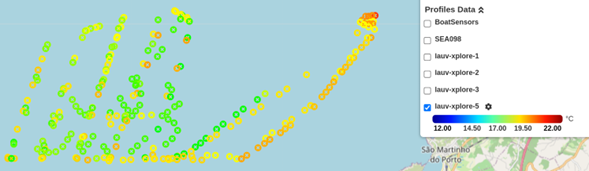
\includegraphics[width=.7\linewidth]{fig/temperatureprofiles.png}
    \caption{INSERT schematic about the 3-day loop}
    \label{fig:temperatureprofiles}
\end{figure}

% The practical implementation of the data cycle in a real-world marine environment introduces several constraints:

% \begin{itemize}
%
% \item \textbf{Communication Limitations}: Low-bandwidth and
%   intermittent communications at sea require that mission planning be
%   sufficiently robust to accommodate long periods of autonomous
%   operation without human intervention.
    
% \item \textbf{Vehicle Constraints}: AUV endurance, payload
%   limitations, navigation precision, and deployment risks all impose
%   restrictions on the feasible operational space and mission duration.

% \item \textbf{Computational Demands}: Real-time generation of
%   uncertainty fields, optimization of paths, and assimilation of
%   collected data must be performed within time windows compatible with
%   daily operational cycles, often under constrained computational
%   resources.

% \item \textbf{Environmental Variability}: Fast-evolving coastal ocean
%   dynamics can introduce discrepancies between forecasted and actual
%   conditions, necessitating robust planning that accounts for forecast
%   uncertainty and adaptivity. \end{itemize}

% This method was deployed and evaluated under the operational framework
% of the FRESNEL project, providing a real-world demonstration of the
% data cycle’s feasibility and benefits in complex coastal environments.


% Distinction Between Onboard and Offboard Predictions:
% \begin{itemize}
%     \item Onboard: Statistical prediction
%     \item Offboard: Numerical prediction
% \end{itemize}

% Rationale and Implementation (including a schematic figure):
% \begin{itemize}
%     \item Why this approach?
%     \item How was it executed?
% \end{itemize}

% Adaptive Sampling Strategy:
% \begin{itemize}
%     \item contraints
%     \item Algorithm used for real-time decision-making
%     \item Criteria for data collection optimization
% \end{itemize}

% Statistical Approach:
% \begin{itemize}
%     \item Techniques applied for uncertainty estimation
%     \item Integration with observational data
% \end{itemize}

%  Numerical Model (HOPS - Harvard Ocean Prediction System):
% \begin{itemize}
%     \item Model configuration and setup
%     \item Data assimilation methods
% \end{itemize}


